\documentclass[12pt,sort&compress]{elsarticle}
\usepackage[utf8]{inputenc}
\usepackage{amsmath}
\usepackage{graphicx}
\usepackage[tableposition=top]{caption}
\usepackage{subcaption}
\usepackage{booktabs}
\usepackage{siunitx}
\usepackage[top=1in,bottom=1in,left=1in,right=1in]{geometry}
\usepackage[pdfborder={0 0 0},colorlinks,allcolors=blue]{hyperref}
\usepackage{txfonts}
\usepackage{setspace}
\usepackage{lineno}

\graphicspath{{figure/}}
\captionsetup[figure]{name=Fig.,labelsep=period}
\def\bibsection{\section*{References}}
\onehalfspacing
\sloppy
\allowdisplaybreaks
\urlstyle{same}
\linenumbers
\journal{TBD}

\begin{document}
\begin{frontmatter}

\title{A Reproducible IEC-Oriented Workflow for Comparative ADCP Tidal Resource Assessment}

\author[sbu]{Jonathan Craig}
\author[sbu]{Hossein Seyedzadeh}
\author{Jiwon Kang}
\author{Elizabeth Hsiao}
\author[sbu]{Ali Khosronejad\corref{cor1}}
\cortext[cor1]{Corresponding author}
\address[sbu]{Department of Civil Engineering, Stony Brook University, Stony Brook, NY 11794, USA}

\begin{abstract}
A reproducible workflow is presented for applying a common tidal-resource analysis to acoustic Doppler current profiler (ADCP) data from different providers and file structures. NOAA CO-OPS station LIS1016 and Verdant Power Stations A and B were processed through shared quality control, principal-flow estimation, tidal-cycle extraction, physical velocity-profile fitting, ensemble-scale variability analysis, and configurable turbine-energy calculations. Verified NOAA deployment metadata converted the LIS1016 cells to 9.41--41.42~m above bed and enabled physical profile analysis alongside the Verdant records. All three datasets exhibited coherent bidirectional flow and repeatable tidal cycles. Comparative single-turbine annual-energy scenarios were 50.8, 121.6, and 139.1~MWh for LIS1016, Station A, and Station B, respectively. The workflow preserves settings, quality-control results, figures, tables, and provenance for each run. The results demonstrate portability across ADCP sources while identifying remaining requirements for IEC-oriented assessment, including independent phase referencing, burst-scale turbulence measurements, long-term resource adjustment, and quantitative uncertainty propagation.
\end{abstract}

\begin{keyword}
Tidal energy \sep Resource assessment \sep Acoustic Doppler current profiler \sep IEC 62600 \sep Velocity profiles \sep Annual energy production
\end{keyword}

\end{frontmatter}
\clearpage
\section{Introduction}
\label{sec:intro}

Marine renewable energy can provide predictable electricity from waves, tides, ocean currents, and rivers. The United States has an estimated marine-energy technical resource of approximately 2300~TWh~yr$^{-1}$, including about 220~TWh~yr$^{-1}$ from tidal currents \cite{nrel_2021}. Converting this technical potential into deployable projects requires site-specific evidence that resolves current magnitude, direction, vertical shear, temporal variability, and the relation between the measured velocity distribution and turbine performance.

The IEC 62600 series provides a common basis for tidal-energy resource assessment and device-performance evaluation. IEC TS 62600-201 organizes resource assessment from feasibility studies toward design-oriented characterization, while IEC TS 62600-200 connects measured current distributions and turbine power curves to energy-production estimates \cite{noauthor_iec_nodate}. These stages depend on measurements with traceable metadata, transparent quality control, documented processing choices, and explicit uncertainty. Acoustic Doppler current profilers (ADCPs) are widely used for this purpose, but provider-specific formats and incomplete metadata can make otherwise comparable analyses difficult to reproduce.

Existing studies demonstrate the importance of principal-flow direction, flood--ebb asymmetry, vertical shear, and turbulence for tidal-device siting and loading \cite{kilcher_tidal_2023,neill_review_2021,sellar_characterisation_2018}. Analysts often address these quantities with separate scripts or notebooks written for one instrument export. That approach complicates review and creates barriers when another ADCP source is introduced. A reusable workflow should separate source-specific ingestion from source-independent calculations and preserve the configuration, quality-control record, figures, and tables associated with each run.

This study develops and demonstrates a configuration-driven ADCP workflow for IEC-oriented tidal resource assessment. It processes a public NOAA Center for Operational Oceanographic Products and Services (CO-OPS) record from station LIS1016 and two Verdant Power deployments in Long Island Sound using a common sequence of preprocessing, flow characterization, profile analysis, variability assessment, and turbine-energy calculations. The comparison evaluates workflow portability and differences among the observed records; because the deployments are neither colocated nor concurrent, it is not a simultaneous intercomparison of instruments or sites. The outputs also support representative inflow conditions for subsequent computational-fluid-dynamics studies associated with the project described by \citet{husoVP2026}.

The remainder of the paper is organized as follows. Section~\ref{sec:methodology} describes the datasets, workflow, hydrodynamic calculations, and energy method. Section~\ref{sec:results} compares data quality, directional structure, tidal cycles, velocity profiles, variability, and energy indicators. Section~\ref{sec:conclusion} summarizes the findings and the remaining requirements for a fuller IEC assessment. Supplementary workflow products and the MATLAB linkage are documented in the appendices.

\section{Methodology}
\label{sec:methodology}

\subsection{Study sites and datasets}
\label{subsec:datasets}

Three ADCP datasets from Long Island Sound were analyzed: NOAA CO-OPS station LIS1016 and Verdant Power Stations A and B. LIS1016 provides a public benchmark near the eastern Long Island Sound study area \cite{coops_map}; the Verdant records provide longer site-specific observations collected in support of tidal-energy development \cite{husoVP2026}. Table~\ref{tab:dataset-summary} lists the retained periods, sampling intervals, bins, and vertical ranges.

\begin{table}[tbp]
\centering
\caption{Datasets retained for the comparative analysis. HAB denotes height above bed.}
\label{tab:dataset-summary}
\resizebox{\textwidth}{!}{%
\begin{tabular}{@{}lllllll@{}}
\toprule
Dataset & Observation period & Interval & Duration & Retained bins & Vertical range & QC outcome \\
\midrule
CO-OPS LIS1016 & 9 Jun--27 Jul 2010 & 6 min & 47.93 d & 17 & 9.41--41.42 m HAB & One missing depth average \\
Verdant Station A & 23 Oct 2024--15 Feb 2025 & 10 min & 114.76 d & 38 & 1.67--20.17 m HAB & Upper five bins excluded \\
Verdant Station B & 23 Oct 2024--15 Feb 2025 & 10 min & 114.88 d & 44 & 1.67--23.17 m HAB & Upper five bins excluded \\
\bottomrule
\end{tabular}}
\end{table}

NOAA metadata identify LIS1016 as an upward-looking ADCP installed 5.18~m above the bed in a pressure-derived water depth of 47.18~m. The cell size is 2.0~m, and the center of bin~1 is 4.23~m above the instrument. NOAA-reported cell depths below the surface, $d_i$, were converted to height above bed as
\begin{equation}
 z_i=47.18-d_i.
 \label{eq:coops-height}
\end{equation}
The resulting heights, 9.41--41.42~m, agree within 0.01~m with the independent geometry calculation
\begin{equation}
 z_i=5.18+4.23+2(i-1).
 \label{eq:coops-geometry}
\end{equation}
This verification permits LIS1016 to be included in the physical profile analysis. For example, the cell at 21.76~m below the surface is bin~9 and lies 25.42~m above the bed.

\subsection{Workflow and quality control}
\label{subsec:workflow}

All datasets were processed with the configuration-driven workflow in Figure~\ref{fig:workflow-overview}. A single JSON file specifies the active source, input path, site metadata, bin exclusions, directional settings, averaging windows, turbine operating speeds, rated power, and power-curve representation. Source-specific readers convert CO-OPS CSV files, Verdant workbooks, or a documented standard CSV into a common table containing time, bin, vertical coordinate, eastward velocity, and northward velocity. All subsequent calculations operate on this representation.

\begin{figure}[tbp]
    \centering
    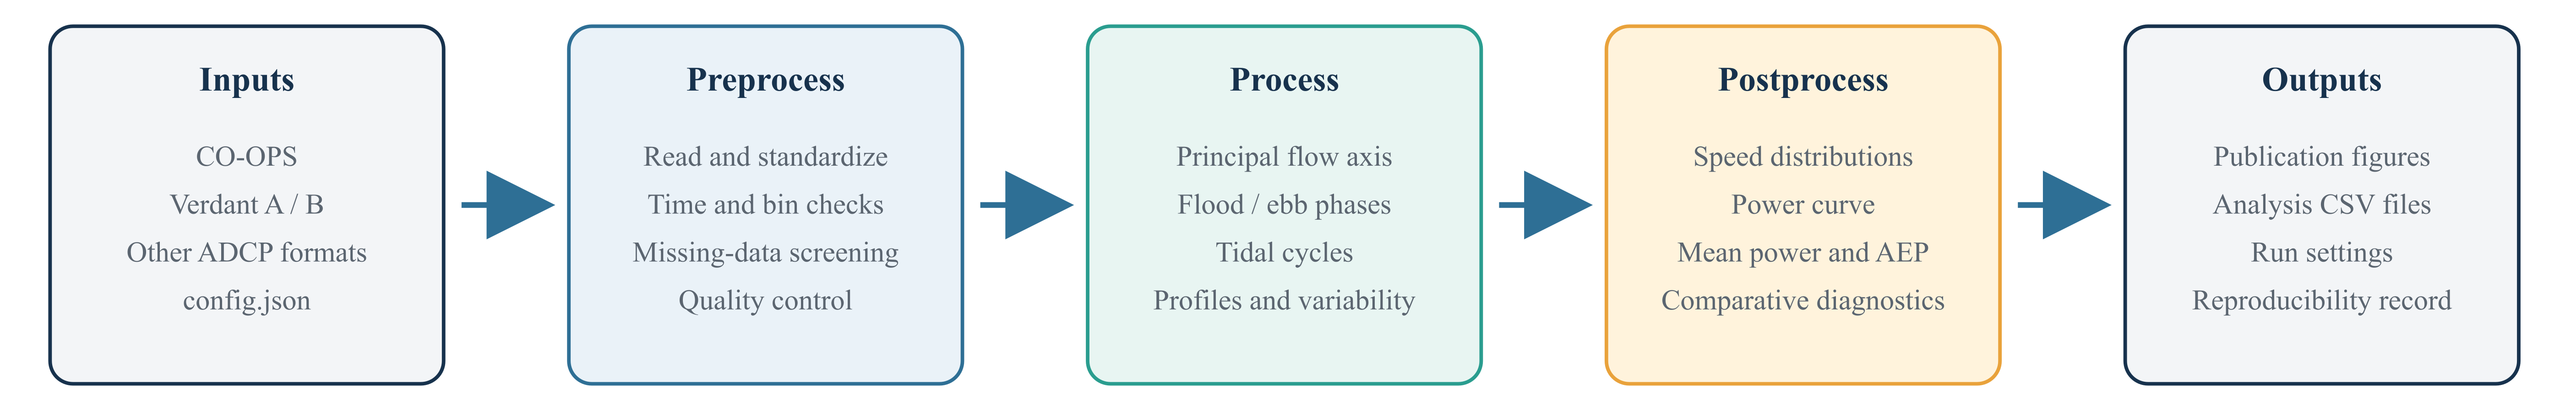
\includegraphics[width=\textwidth]{figure/workflow_overview.png}
    \caption{Configuration-driven workflow for applying an IEC-oriented tidal resource assessment to different ADCP sources. User inputs and turbine assumptions are defined once, while the backend performs preprocessing, analysis, postprocessing, and reproducible export.}
    \label{fig:workflow-overview}
\end{figure}

Preprocessing validates timestamps, bin identifiers, units, true bearings, depth metadata, and source-specific geometry. Identical duplicates are removed; conflicting overlaps are rejected; velocities that are missing or exceed the configured limit remain missing rather than being reclassified as slack. Bin coverage is evaluated before vector depth averages are calculated. Sampling gaps define separate analysis blocks so smoothing, cycle extraction, and time weighting do not bridge unsupported intervals.

Every run exports the effective settings, input-file hashes, quality-control summaries, processed tables, figures, and a run log. The source adapters therefore remain separate from the scientific calculations, allowing a new ADCP format to be added without duplicating the analysis.

\subsection{Principal flow, tidal cycles, and velocity profiles}
\label{subsec:flow-profiles}

The dominant bidirectional current axis was estimated from the depth-averaged horizontal velocity. For the doubled-angle formulation, the axial bearing is
\begin{equation}
\theta_{\mathrm{axis}}=\frac{1}{2}\operatorname{atan2}
\left(\left\langle\sin 2\theta\right\rangle,
\left\langle\cos 2\theta\right\rangle\right).
\label{eq:principal-axis}
\end{equation}
The implemented principal-component alternative determines the same type of undirected axis from the covariance of the eastward and northward components. Either method has a 180$^{\circ}$ ambiguity. The axis end nearest an independent flood-direction reference is labeled flood, and the opposite end is labeled ebb. Without an independent phase reference, the physically supportable labels are positive and negative principal flow.

Velocity vectors were projected onto the oriented axis. The along-axis series was smoothed only within continuous analysis blocks and classified as flood, ebb, or slack. The slack threshold equaled the turbine cut-in speed, 0.4~m~s$^{-1}$ in the present runs. Flood and ebb events were separated at interpolated zero crossings. Accepted events between 6 and 18 hours were mapped to a normalized cycle coordinate, ensemble averaged, and represented with a periodic cosine fit. Fit quality was described by amplitude, $R^2$, and root-mean-square error (RMSE).

Phase-mean physical profiles were fitted with a normalized power law,
\begin{equation}
\frac{\overline{u}(z)}{U}=\left(\frac{\eta}{\beta}\right)^{1/\alpha},
\qquad \eta=\frac{z}{h},
\label{eq:power-law}
\end{equation}
and a near-bed logarithmic law,
\begin{equation}
\overline{u}(z)=\frac{u_*}{\kappa}\ln\left(\frac{z}{z_0}\right),
\label{eq:log-law}
\end{equation}
where $z$ is height above bed, $h$ is water depth, $U$ is the mean velocity over the retained cells, $\alpha$ and $\beta$ are fitted power-law parameters, $u_*$ is friction velocity, $\kappa=0.41$, and $z_0$ is fitted roughness length. Power-law fits used all retained physical cells. Logarithmic fits were limited to the configured near-bed fraction and required at least three cells. The LIS1016 limit was set to $z/h\leq0.30$ so its lowest three cells were included without automatic expansion. Record-peak normalized profiles were retained as separate diagnostics and were not substituted for phase-mean physical fits.

\subsection{Flow variability}
\label{subsec:variability-method}

Gap-aware residuals were calculated after removal of a slowly varying streamwise signal. For each phase, residual intensity was defined as
\begin{equation}
I_u=100\frac{\sigma_{u'}}{\overline{|u|}},
\label{eq:residual-intensity}
\end{equation}
where $\sigma_{u'}$ is the sample standard deviation of the resolved streamwise residual and $\overline{|u|}$ is the corresponding mean absolute streamwise velocity. An optional correction subtracts a supplied Doppler-noise variance,
\begin{equation}
I_{u,\mathrm{corr}}=100\frac{\sqrt{\max(\sigma_{u'}^2-\sigma_{\mathrm{noise}}^2,0)}}{\overline{|u|}}.
\label{eq:noise-correction}
\end{equation}
The comparative runs used $\sigma_{\mathrm{noise}}=0.1$~m~s$^{-1}$. This was a configured assumption rather than an instrument-specific spectral estimate. Because the native observations are 6- or 10-minute ensembles, these statistics describe ensemble-scale variability and are not interpreted as validated burst-scale turbulence intensity.

\subsection{Power and annual energy production}
\label{subsec:energy-method}

Energy calculations used the time-weighted speed distribution at the selected hub bin. Each observation was assigned support from the native sampling interval, with support capped across data gaps. The same turbine curve was applied to all datasets: cut-in speed 0.4~m~s$^{-1}$, rated speed 1.5~m~s$^{-1}$, cut-out speed 3.2~m~s$^{-1}$, and rated power 110~kW. Mean power was obtained by weighting the power associated with each speed interval by its observed probability. Annual energy production and capacity factor were calculated as
\begin{equation}
\mathrm{AEP}=\overline{P}\,T_{\mathrm{year}}A,
\qquad
\mathrm{CF}=\frac{\overline{P}}{P_{\mathrm{rated}}},
\label{eq:aep}
\end{equation}
where $T_{\mathrm{year}}=8766$~h and availability $A=1$ for the comparative scenario. These short-record, single-turbine estimates exclude long-term adjustment, array interactions, electrical losses, environmental curtailment, and downtime.

\subsection{Uncertainty and reproducibility}
\label{subsec:uncertainty}

Principal uncertainty sources include instrument accuracy, directional alignment, vertical-coordinate metadata, selected bins, depth averaging, the independent flood reference, the assumed noise level, deployment duration, and the turbine power curve. The workflow records these inputs and their quality-control outcomes, but a combined quantitative uncertainty budget has not yet been propagated through the resource and energy results. The outputs are therefore reproducible comparative estimates and inputs to subsequent IEC-oriented assessment, rather than a declaration of full IEC conformity.

\section{Results and Discussion}
\label{sec:results}

\subsection{Data quality and source comparison}
\label{subsec:data-quality-results}

The common quality-control procedure retained 195,558 depth-resolved observations across 17 cells for LIS1016, 627,988 observations across 38 cells for Station A, and 727,848 observations across 44 cells for Station B. No identical duplicates or invalid-velocity rows occurred in the retained inputs. One LIS1016 timestamp lacked a valid depth average; the Verdant depth-averaged series were complete after their upper five cells were excluded.

The Verdant records cover approximately 2.4 times the LIS1016 duration and consequently contain more accepted tidal cycles. All three datasets now have confirmed physical heights above bed, so each supports phase-mean profile fitting. The nonconcurrent records serve different comparison roles: LIS1016 tests the public CO-OPS ingestion path, while Stations A and B test the Verdant workbook adapter and site-specific geometry. Differences among the records represent their observed periods and locations and should not be interpreted as simultaneous instrument validation.

\subsection{Flow direction and tidal cycles}
\label{subsec:flow-results}

Figure~\ref{fig:principal-flow-comparison} shows a stable bidirectional axis in every dataset. Flood-facing principal bearings were 245.1$^{\circ}$T for LIS1016, 252.2$^{\circ}$T for Station A, and 255.5$^{\circ}$T for Station B. The two Verdant axes differ by 3.3$^{\circ}$, whereas LIS1016 is rotated by approximately 7--10$^{\circ}$ relative to them. The offset may reflect channel geometry, deployment location, or directional uncertainty; the noncolocated records do not support attributing it to bathymetry alone.

\begin{figure}[tbp]
\centering
\begin{subfigure}[t]{0.98\textwidth}\centering
\includegraphics[width=\linewidth]{figure/coops/principal_flow_diagnostics.png}
\caption{CO-OPS LIS1016}
\end{subfigure}
\medskip
\begin{subfigure}[t]{0.98\textwidth}\centering
\includegraphics[width=\linewidth]{figure/verdantA/principal_flow_diagnostics.png}
\caption{Verdant Station A}
\end{subfigure}
\medskip
\begin{subfigure}[t]{0.98\textwidth}\centering
\includegraphics[width=\linewidth]{figure/verdantB/principal_flow_diagnostics.png}
\caption{Verdant Station B}
\end{subfigure}
\caption{Principal-flow diagnostics for the three ADCP records. The common method resolves the bidirectional axis before the opposing phases are labeled using the independent flood reference.}
\label{fig:principal-flow-comparison}
\end{figure}

The polar comparison in Figure~\ref{fig:polar-comparison} confirms nearly antiparallel phase-mean directions. Flood and ebb directions were 244.5$^{\circ}$T and 67.4$^{\circ}$T at LIS1016, 252.3$^{\circ}$T and 72.9$^{\circ}$T at Station A, and 255.4$^{\circ}$T and 76.9$^{\circ}$T at Station B. Each pair deviated by less than 3$^{\circ}$ from exact opposition. Mean flood and ebb speeds were 0.693 and 0.723~m~s$^{-1}$ at LIS1016, 0.795 and 0.839~m~s$^{-1}$ at Station A, and 0.870 and 0.839~m~s$^{-1}$ at Station B. Station B had the largest flood peak, 1.567~m~s$^{-1}$; Station A and B ebb peaks were similar at 1.487 and 1.497~m~s$^{-1}$.

\begin{figure}[tbp]
\centering
\begin{subfigure}[t]{0.47\textwidth}\centering
\includegraphics[width=\linewidth]{figure/coops/tidal_velocity_polar.png}
\caption{CO-OPS LIS1016}
\end{subfigure}\hfill
\begin{subfigure}[t]{0.47\textwidth}\centering
\includegraphics[width=\linewidth]{figure/verdantA/tidal_velocity_polar.png}
\caption{Verdant Station A}
\end{subfigure}
\medskip
\begin{subfigure}[t]{0.47\textwidth}\centering
\includegraphics[width=\linewidth]{figure/verdantB/tidal_velocity_polar.png}
\caption{Verdant Station B}
\end{subfigure}
\caption{Tidal velocity magnitude and direction. The black line denotes the bidirectional principal axis; colored arrows show phase-mean flood and ebb bearings.}
\label{fig:polar-comparison}
\end{figure}

The normalized-cycle analysis in Figure~\ref{fig:cycle-comparison} retained 91 events for LIS1016, 220 for Station A, and 221 for Station B. Fitted amplitudes were 0.858, 1.033, and 1.087~m~s$^{-1}$, respectively. Corresponding $R^2$ values were 0.997, 0.988, and 0.992, and RMSE values were 0.031, 0.079, and 0.069~m~s$^{-1}$. A repeatable dominant cycle is therefore resolved in each record. The broader event spread at the Verdant sites shows variability not represented by the ensemble-mean cosine curve. These finite deployments do not replace long-term harmonic analysis or seasonal adjustment.

\begin{figure}[tbp]
\centering
\begin{subfigure}[t]{0.47\textwidth}\centering
\includegraphics[width=\linewidth]{figure/coops/tidal_cycles.png}
\caption{CO-OPS LIS1016}
\end{subfigure}\hfill
\begin{subfigure}[t]{0.47\textwidth}\centering
\includegraphics[width=\linewidth]{figure/verdantA/tidal_cycles.png}
\caption{Verdant Station A}
\end{subfigure}
\medskip
\begin{subfigure}[t]{0.47\textwidth}\centering
\includegraphics[width=\linewidth]{figure/verdantB/tidal_cycles.png}
\caption{Verdant Station B}
\end{subfigure}
\caption{Phase-normalized tidal cycles derived from principal velocity. Positive and negative velocities denote the opposing flood and ebb phases on a common cycle coordinate.}
\label{fig:cycle-comparison}
\end{figure}

\subsection{Profiles, shear, and variability}
\label{subsec:profile-results}

Figure~\ref{fig:profile-comparison} compares normalized record-peak profile diagnostics, with ebb shown as negative velocity and flood as positive velocity. These plots demonstrate phase-dependent shear, but their annotations describe selected peak profiles. The phase-mean physical fits used for quantitative comparison were calculated separately with verified height-above-bed coordinates.

\begin{figure}[tbp]
\centering
\begin{subfigure}[t]{0.47\textwidth}\centering
\includegraphics[width=\linewidth]{figure/coops/Velocity_profiles.png}
\caption{CO-OPS LIS1016}
\end{subfigure}\hfill
\begin{subfigure}[t]{0.47\textwidth}\centering
\includegraphics[width=\linewidth]{figure/verdantA/Velocity_profiles.png}
\caption{Verdant Station A}
\end{subfigure}
\medskip
\begin{subfigure}[t]{0.47\textwidth}\centering
\includegraphics[width=\linewidth]{figure/verdantB/Velocity_profiles.png}
\caption{Verdant Station B}
\end{subfigure}
\caption{Normalized record-peak flood and ebb profile diagnostics retained from the postprocessing workflow. The plotted fit parameters describe selected peak profiles and are distinct from the phase-mean physical fits reported in the text.}
\label{fig:profile-comparison}
\end{figure}

For LIS1016, the corrected physical coordinate produced power-law parameters $\alpha=1.67$, $\beta=0.523$, and $R^2=0.974$ for ebb and $\alpha=2.88$, $\beta=0.510$, and $R^2=0.988$ for flood. Three-cell log-law fits within $z/h\leq0.30$ yielded $R^2=0.998$ for ebb and approximately 1.000 for flood. The associated $u_*$ values were 0.0797 and 0.0561~m~s$^{-1}$, and fitted $z_0$ values were 1.008 and 0.219~m. The large roughness lengths and narrow fitting interval show that these parameters should be treated as model diagnostics rather than direct measurements of bed roughness.

Station A power-law fits produced $\alpha=4.44$ and $\beta=0.401$ for ebb and $\alpha=7.98$ and $\beta=0.392$ for flood, with $R^2=0.965$ and 0.999. Station B produced $\alpha=4.53$ and $\beta=0.404$ for ebb and $\alpha=6.22$ and $\beta=0.398$ for flood, with $R^2=0.987$ and 0.989. Verdant log-law fits had $R^2>0.997$ for both phases. Fitted friction velocities ranged from 0.0358 to 0.0386~m~s$^{-1}$ at Station A and from 0.0466 to 0.0493~m~s$^{-1}$ at Station B; roughness lengths ranged from 0.00161 to 0.00205~m and from 0.00859 to 0.01054~m, respectively. These results support phase-specific profile descriptions, although fitted parameters remain sensitive to the selected cells and model form.

Figure~\ref{fig:variability-comparison} shows the depth-dependent variability indicator retained from the original postprocessing, while Table~\ref{tab:comparative-results} reports consolidated streamwise residual intensity. Raw flood and ebb residual intensities were 17.3\% and 15.9\% at LIS1016, 17.1\% and 17.4\% at Station A, and 16.5\% and 18.4\% at Station B. After subtraction of the configured noise variance, they were 9.5\% and 7.7\%, 11.5\% and 12.6\%, and 11.8\% and 14.0\%, respectively.

\begin{figure}[tbp]
\centering
\begin{subfigure}[t]{0.47\textwidth}\centering
\includegraphics[width=\linewidth]{figure/coops/TI_original_profiles.png}
\caption{CO-OPS LIS1016}
\end{subfigure}\hfill
\begin{subfigure}[t]{0.47\textwidth}\centering
\includegraphics[width=\linewidth]{figure/verdantA/TI_original_profiles.png}
\caption{Verdant Station A}
\end{subfigure}
\medskip
\begin{subfigure}[t]{0.47\textwidth}\centering
\includegraphics[width=\linewidth]{figure/verdantB/TI_original_profiles.png}
\caption{Verdant Station B}
\end{subfigure}
\caption{Depth-dependent variability resolved at each dataset's native ensemble interval. The displayed diagnostic and consolidated residual intensity use different detrending and normalization conventions and should not be interpreted as burst-scale turbulence measurements.}
\label{fig:variability-comparison}
\end{figure}

The difference between the plotted legacy indicator and the consolidated residual metric demonstrates sensitivity to detrending and denominator choice. In some legacy calculations, the assumed noise variance exceeded the resolved fluctuation variance, so corrected variance was clipped to zero. Instrument-specific noise characterization and burst-mode measurements are required before these outputs can support definitive IEC turbulence statistics.

\subsection{Resource and energy results}
\label{subsec:energy-results}

Figure~\ref{fig:resource-energy-inputs} compares the time-weighted hub-bin distributions and the common turbine curve. Mean profile speed exceeded the 0.4~m~s$^{-1}$ operating threshold during 71.2\% of the LIS1016 record, 78.8\% of the Station A record, and 77.2\% of the Station B record. Although the two Verdant operating fractions were similar, Station B contained more probability at higher flood velocities. Operating duration alone therefore does not determine energy yield; the entire distribution must be considered relative to the nonlinear power curve.

\begin{figure}[tbp]
\centering
\begin{subfigure}[t]{0.47\textwidth}\centering
\includegraphics[width=\linewidth]{figure/coops/hub_velocity_probability.png}
\caption{CO-OPS LIS1016}
\end{subfigure}\hfill
\begin{subfigure}[t]{0.47\textwidth}\centering
\includegraphics[width=\linewidth]{figure/verdantA/hub_velocity_probability.png}
\caption{Verdant Station A}
\end{subfigure}
\medskip
\begin{subfigure}[t]{0.47\textwidth}\centering
\includegraphics[width=\linewidth]{figure/verdantB/hub_velocity_probability.png}
\caption{Verdant Station B}
\end{subfigure}\hfill
\begin{subfigure}[t]{0.47\textwidth}\centering
\includegraphics[width=\linewidth]{figure/verdantB/turbine_power_curve.png}
\caption{Configured turbine power curve}
\end{subfigure}
\caption{Hub-bin velocity distributions and the common turbine power curve used for the comparative energy scenarios. Turbine thresholds and power-curve values are supplied through the global configuration file.}
\label{fig:resource-energy-inputs}
\end{figure}

Table~\ref{tab:comparative-results} consolidates the principal indicators. Mean turbine power was 5.79~kW for LIS1016, 13.88~kW for Station A, and 15.87~kW for Station B. Annualization produced 50.8, 121.6, and 139.1~MWh, corresponding to capacity factors of 5.27\%, 12.61\%, and 14.42\%. Station B's higher estimate is consistent with its larger mean and peak flood speeds and its greater probability within the productive portion of the configured curve.

\begin{table}[tbp]
\centering
\caption{Principal hydrodynamic and energy indicators. Directions are degrees true; residual intensity describes variability resolved at the native ensemble interval.}
\label{tab:comparative-results}
\begin{tabular}{@{}lccc@{}}
\toprule
Metric & CO-OPS & Verdant A & Verdant B \\
\midrule
Flood-facing principal bearing ($^\circ$) & 245.1 & 252.2 & 255.5 \\
Mean flood speed (\si{\metre\per\second}) & 0.693 & 0.795 & 0.870 \\
Mean ebb speed (\si{\metre\per\second}) & 0.723 & 0.839 & 0.839 \\
Peak flood speed (\si{\metre\per\second}) & 1.103 & 1.310 & 1.567 \\
Peak ebb speed (\si{\metre\per\second}) & 1.184 & 1.487 & 1.497 \\
Mean flood direction ($^\circ$) & 244.5 & 252.3 & 255.4 \\
Mean ebb direction ($^\circ$) & 67.4 & 72.9 & 76.9 \\
Accepted tidal cycles & 91 & 220 & 221 \\
Cycle amplitude (\si{\metre\per\second}) & 0.858 & 1.033 & 1.087 \\
Cycle-fit $R^2$ & 0.997 & 0.988 & 0.992 \\
Flood residual intensity (\%) & 17.3 & 17.1 & 16.5 \\
Ebb residual intensity (\%) & 15.9 & 17.4 & 18.4 \\
Mean turbine power (\si{\kilo\watt}) & 5.79 & 13.88 & 15.87 \\
Annual energy (\si{\mega\watt\hour}) & 50.8 & 121.6 & 139.1 \\
Capacity factor (\%) & 5.27 & 12.61 & 14.42 \\
\bottomrule
\end{tabular}
\end{table}

The annual-energy values extrapolate approximately 48--115 days to 8766 hours and assume 100\% availability. They exclude interannual variability, long-term tidal adjustment, turbine-array interactions, electrical losses, environmental constraints, and downtime. They are comparative scenarios rather than certified long-term or project-level AEP estimates.

\subsection{IEC implications and limitations}
\label{subsec:iec-results}

Table~\ref{tab:iec-traceability} maps the implemented analyses to major needs of an IEC-oriented resource assessment. The workflow demonstrates reproducible quality-control reporting, principal-flow characterization, tidal-cycle extraction, physical profile fitting, velocity-distribution analysis, configurable turbine calculations, and traceable export for multiple ADCP formats.

\begin{table}[tbp]
\centering
\caption{IEC-oriented coverage of the workflow and principal limitations of the current implementation.}
\label{tab:iec-traceability}
\small
\begin{tabular}{p{0.18\textwidth}p{0.27\textwidth}p{0.25\textwidth}p{0.19\textwidth}}
\toprule
Assessment topic & Workflow implementation & Evidence produced & Current status \\
\midrule
Data quality and metadata & Sampling, bin, missing-data, geometry, and coverage checks & QC tables, run logs, and retained-bin records & Demonstrated \\
Principal flow and direction & PCA or doubled-angle axis, phase statistics, polar plots, and cycles & Principal-axis and phase-direction outputs & Independent phase reference required \\
Vertical shear & Flood and ebb physical power-law and logarithmic fits & Profile diagnostics and fit parameters & Demonstrated for all three records \\
Flow variability & Ensemble residual and depth-dependent intensity calculations & Raw and noise-corrected variability outputs & Burst-scale turbulence unavailable \\
Velocity distribution and energy & Hub-bin distribution combined with a configurable power curve & Mean power, AEP, capacity factor, and energy contribution & Comparative scenario \\
Uncertainty and reporting & Saved configuration, hashes, outputs, and processing records & Reproducible run products & Quantitative uncertainty budget required \\
\bottomrule
\end{tabular}
\end{table}

Four limitations control interpretation. First, a principal axis has a 180$^{\circ}$ ambiguity, so physical flood and ebb labels require an independent directional or tidal-phase reference. Second, profile parameters depend on verified geometry and the selected fitting interval; the three-cell LIS1016 log-law result is especially localized. Third, the 6- and 10-minute ensembles do not resolve burst-scale turbulence, and the noise correction uses a supplied standard deviation rather than an instrument-specific spectral estimate. Fourth, the short-record energy scenarios lack long-term adjustment and a propagated uncertainty budget.

The framework organizes evidence for IEC-oriented assessment but does not establish IEC conformity by itself. Further development should add automated tidal-phase referencing, instrument-specific uncertainty models, burst-mode turbulence measurements, long-term resource adjustment, and uncertainty propagation into AEP. Within the present limits, consistent processing of CO-OPS and Verdant inputs demonstrates that one workflow can support comparative resource characterization without separate analysis code for each provider.

\section{Conclusion}
\label{sec:conclusion}

A single configuration-driven workflow was developed to process NOAA CO-OPS, Verdant Power, and standardized ADCP records through common preprocessing, hydrodynamic analysis, and postprocessing steps. Source adapters preserve provider-specific ingestion while the scientific calculations use a shared data structure. Each run records its settings, quality-control results, processed tables, figures, and provenance, reducing ambiguity created by separate site-specific scripts.

Application to LIS1016 and Verdant Stations A and B resolved coherent bidirectional axes and repeatable tidal cycles across all three records. Verified NOAA metadata converted LIS1016 cells to 9.41--41.42~m above bed and enabled physical power-law and near-bed logarithmic fits alongside the Verdant datasets. The Verdant records exhibited larger cycle amplitudes and higher comparative energy estimates than LIS1016, with Station B producing the largest mean-power and AEP scenario. These differences describe the observed records and should not be interpreted as a concurrent site ranking.

The workflow covers quality control, directional analysis, vertical shear, velocity distributions, and configurable energy calculations needed for an IEC-oriented resource study. Its present limits are equally important: the records do not resolve burst-scale turbulence, the noise correction is assumed, AEP is extrapolated from short deployments, and a combined uncertainty budget has not been propagated. Addressing these limitations is necessary before the outputs can support a formal conformity claim or project-level energy forecast.

\section*{Acknowledgements}
\addcontentsline{toc}{section}{Acknowledgements}
This study was supported by Verdant Power Inc. Partial support was provided by the U.S. Department of Energy's Hydropower and Hydrokinetic Office under Award No.~DE-EE0009450. The views expressed herein do not necessarily represent those of the U.S. Department of Energy or the United States Government.

\section*{Data and Code Availability}
\addcontentsline{toc}{section}{Data and Code Availability}
The analysis workflow and supporting source code are available through the project \href{https://github.com/hosseinsz93/Verdant-SBU-tidal-project}{GitHub repository}. NOAA CO-OPS observations and metadata are publicly available through NOAA Tides and Currents. Access to Verdant Power source measurements is subject to the project's data-sharing conditions; processed products should be distributed only where those conditions permit.

\appendix
\section{Supplementary workflow outputs}
\label{app:outputs}

The main text presents outputs required for the comparative argument. The workflow also retains source-specific time series, velocity-component plots, current roses, phase statistics, empirical probability distributions, energy-contribution plots, annual-event comparisons, and run-level quality-control tables. These products remain available for diagnostic review without duplicating their descriptions in the main Results and Discussion section. Table~\ref{tab:supplementary-outputs} summarizes their intended use.

\begin{table}[tbp]
\centering
\caption{Supplementary workflow products retained for diagnostic review.}
\label{tab:supplementary-outputs}
\begin{tabular}{@{}p{0.28\textwidth}p{0.62\textwidth}@{}}
\toprule
Product & Intended interpretation \\
\midrule
Time series and components & Review gaps, phase classification, directional sign, and individual events \\
Flow summaries and statistics & Review phase distributions, extrema, and descriptive statistics \\
Current roses & Inspect the joint distribution of true bearing and current speed \\
Probability and contribution plots & Trace energy estimates to velocity probabilities and turbine-curve intervals \\
Annual-event comparison & Compare optional CO-OPS prediction events separately from measured ADCP resource calculations \\
Run log and QC tables & Reproduce the effective settings, inputs, exclusions, and retained observations \\
\bottomrule
\end{tabular}
\end{table}

\section{Supplementary MATLAB processing}
\label{app:matlab}

For supplementary tidal analyses, measurements for each depth and month can be exported as separate CSV files and processed with the associated MATLAB routines. Because the original CO-OPS filenames identify the station and depth but do not provide every descriptor required by the legacy MATLAB algorithms, exported files may require clear depth- and month-specific names before processing. These routines complement the tidal analyses and CFD simulations presented by \citet{husoVP2026} and are available through the project \href{https://github.com/hosseinsz93/Verdant-SBU-tidal-project}{GitHub repository}.

{\small
\bibliographystyle{elsarticle-num-names}
\bibliography{main}
}
\end{document}
